\documentclass{article}
\usepackage[utf8]{inputenc}
\usepackage{graphicx}

\title{Connectivity, Language, and Meaning}
\author{MCB C61 with Professor David Presti \\ \\ Benjamin Lee}
% \date{8 March 2018}

\begin{document}

\maketitle

\textbf{Key Concepts:}
\begin{itemize}
    \item Cortical layers and connectivity
    \item Hemispheric assymmetry
    \item Aphasia: Broca's, Wenicke's
    \item Broca's area, Wenicke's area 
    \item Wada Test
    \item Language lateralization and handedness
    \item Linguistic mirror neurons
    \item Roger Sperry, corpus collosotomy, split-brain patients
    \itm Lateralization of function
    \item Neural correlates of consciousness (NCC) 
    \item Cortical neuropil 
    \item Walter Freeman
    \item Ephaptic coupling
\end{itemize}

\newpage

\section{Cortical Layers and Connectivity}
All mammals have \textbf{layered} cerebral cortex containing similar neural circuitry. \\
There is a \textbf{local interconnectivity} within and between cortical layers and there is a long-range connectivity between widely separated regions of the cerebrum \\

\noindent Ex: neurons in the occipital lobes form connections with neurons in the frontal lobes, and vice versa \\

\noindent Extensive connectivity going in both directions between the crebral cortex and many subcortical structures: thalamus, amygdala, hypothalamus, substantia nigra, ventral tegmentum, locus coeruleus, raphe nuclei, etc. \\

\section{Hemispheric Assymmetry}
The two hemispheres of the human cerebral cortex appear roughly identical; however, there are differences in function between the two sides of the brain (\textbf{lateralization of function}). 
\begin{itemize}
    \item \textbf{Anosognosia} ("lack of insight") illustrates the concept of lateralization of cerebral cortex function
        \subitem Often associated with lesions to the right cerebral hemisphere with damage to the left cerebral hemisphere
    \item \textbf{Prosopagnosia} more associated with right than with left-hemisphere lesions
    \item Classic function associated with hemispheric specialization is \textbf{language}: the capacity to communicate using signs, sounds, and gestures that have understood meanings
    \item Language is the one of the most elaborate and sophisticated aspects of human behavior
    \item Ex: Three words: I, know, you \\ 
    "I know"\\ 
    "I know you know"\\
    "I know you know I know" \\
    "I know you know I know you know". \\
    \item Build sentences of unending complexity, where the meaning changes in subtle ways 
    \item Syntax and semantics determine the construction of meaningful phrases and sentences. 
\end{itemize}

\section{Broca's Area and Wernicke's Area}

Paul Broca (1824-1880) a French physician who pioneered in investigating the neuroanatomy of language

\noindent Carl Wernicke (1848 - 1905) a German physician. 

\subsection{Aphasia's}
\textbf{Definition:} Neurologically based impairment in language function \\

\noindent \textbf{Broca's Aphasia:}
\begin{itemize}
    \item Associated the capacity to speak
    \item Broca's aphasia is used to describe the condition in which a person has problems with producing spoken and written language
    \item Language production is associated with lesions in the \textbf{left frontal premotor area} of the brain, known as \textbf{Broca's area}
    \item This aphasia is a \textbf{motor apraxia} specific to language
        \subitem Although they can move their arms, hands, mouth, and tongue, they cannot organize their movements to produce written or spoken language. 
    \item Motor aparaxias associated with lesions to frontal premotor areas
\end{itemize}

\noindent \textbf{Wernicke's Aphasia}: 
\begin{itemize}
    \item Problem with the comprehension of spoken and written language
    \item Vision and hearing are unimpaired, a patient with Wernicke's aphasia cannot understand (cannot interpret the meaning of) spoken and written language
    \item Associated with lesions in \textbf{posterior left temporal lobe} that has come to be called \textbf{Wernicke's area}
    \item \textbf{Sensory agnosia} specific to language 
    \item Sensory agnosias associated with lesions in cortical region where temporal, parietal and occipital lobes come together. 
    \item This area of brain involved in integration and interpretation of a variety of different kinds of sensory information coming from visual, auditory and tactile channels
    \item Often can write or speak, but the language is incomprehensible 
\end{itemize}

Findings of Broca and Wernicke in 19th century suggested that language regions of the brain are primarily located in the left cerebral hemisphere. Both hemispheres are associated with language, but the left side is dominant for language production. \\

\section{Wada Test}
When patients suffer from severe seizure disorders, small regions of the cerebral cortex can be pinpointed as the loci of generation of seizures. Procedures have been developed to surgically locate and remove these areas, and since they are often near the temporal region, surgeons must take great care not to damage the language centers of the brain. \\ 

\noindent In the 1940's, neurlogist Juhn Wada developed a presurgical test for determining the dominant hemisphere for language. 

\begin{itemize}
    \item Injects a small dose of sedative-hypnotic barbiturate drug, such as amobarbital, into either the right or left carotid artery
    \item Patient is then asked to count: one, two, three, etc
    \item In seconds, the barbiturate infuses the cortex on one side of the brain, causing widespread inhibition of neuronal activity
    \item If the drug reaches a part of the brain involved with language production, the patient immediately stops counting and can only resume when the drug dissipates
    \item If it goes in the non-language-dominant hemisphere, then as the barbiturate takes effect, there is a slight hesitation due to the effects felt, but the counting is then resumed following
\end{itemize}
These days it has been replaced with noninvasive brain imaging procedures such as MEG and fMRI

\section{Language Lateralization and Handedness}
We can determine the lateralization of language with our imaging techniques and Wada tests. 

\begin{itemize}
    \item Most people have left-hemisphere language dominance
    \item However, there is a relationship between handedness and lateralization of language
    \item \textbf{Right-handed people:} 97\% left-hemisphere language dominance and 3\% right-hemisphere language dominance
    \item \textbf{Non-right-handed (left or ambidextrous):} 70\% left-hemisphere language dominance and 15\% right-hemisphere language dominance and 15\% have substantial language control by both hemispheres
\end{itemize}

\newpage
\noindent \textbf{Cortical Path of Language:}
\begin{itemize}
    \item Language is first heard, so it activates the \textbf{auditory cortex (A1)} first
    \item If there is \textbf{meaning} to the words that are begin heard, then \textbf{Wernicke's area} also become active
    \item Even if the language isn't understood, Wernicke's area still lights up
    \item If the language is \textbf{understood}, then \textbf{Broca's area} also becomes active
    \item Broca's area is not restricted to speaking and writing but is also relevant for listening, reading, and understanding language
    \item \textbf{Linguistic Mirror Neurons:} Neurons in Broca's area are premotor mirror neurons, active when observing (reading, listening and understanding) language, as well as generating (writing and speaking) language
    \item Mirror neurons connect perception with action in a direct way
    \item Gives meaning to perceptions and actions 
\end{itemize}


\section{Roger Sperry and Split-Brains}
1960's-1970's revealed much information about lateralization of cerebral function for a variety of human behaviors. \\

Sperry worked with patients who suffered from severe epilepsy, in which seizures propagated across the \textbf{corpus callosum} from one hemisphere to the other, disabling large parts of the brain. \\ 

\noindent\textbf{Corpus Collosotomy:}
\begin{itemize}
    \item Procedure of severing the corpus callosum, disconnecting direct neural communication between the two hemispheres of the cerebral cortex
    \item Substantially reduced the frequency and intensity of seizures and may have been a life-saving surgery
    \item Patients referred to as split-brain patients (brain literally split in two)
    \item \textbf{Corpus callosum:} large bundle of axons connecting the right and left hemispheres of cerebral cortex in mammalian brains
        \subitem spans several centimeters and consists of 200 million neurons
\end{itemize}

\noindent \textbf{Split-Brain Experiments:}
\begin{itemize}
    \item Sperry's experiment: patient sat in a chair and looked at the center of a small screen. 
    \item Brief flash of pictures or words to either patient left or right visual field
    \item Visual information goes to the person's left cerebral hemisphere(right visual field), he is asked to report what he saw, and answers correctly
    \item If picture flashed in patient's left visual field and asked to report, he can't say. 
    \item He can point out the object with his left hand (because left side controlled by right-hemisphere)
    \item Can't say because left visual field went into nonspeaking right hemisphere
    \item Sometimes they will make up a story
    \item \textbf{Lateralization of Function} between left and right hemisphere is exemplified in these experiments and we see the corpus collosum as a transport of information between the hemispheres
\end{itemize}

\begin{figure}[htp]
\centering
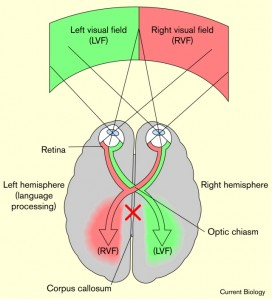
\includegraphics[width= 6cm]{images/split-brain-Sperry.jpg}
\caption{Sperry's Split Brain Experiment}
\label{fig: split-brain}
\end{figure}

\newpage
\subsection{Psycological Defenses}
\textbf{Definition:} \textbf{Sigmund Freud (1856-1939)} and others described this as cognitive strategies to protect ourselves from experiencing thoughts and feelings that might provoke anxiety or otherwise bothersome feelings. Dubbed \textbf{Freudian defenses} \\

Such strategies may be stories (rationalization, projection, reaction, formation, etc) or out-and-out forgetting (repression, suppression). These are out of our awareness(unconscious) and not aware of our motivations for defensive action. \\

\begin{itemize}
    \item Left-hemisphere: superior to the right for language comprehension and expression, numeric reasoning and arithmetic calculation and visual detail
    \item Right-hemisphere: superior to the left for nonverbal aspects of communication, such as linguistic prosody (rhythm, intonation), tone of voice, and body language, and for visual perspective and larger-scale spatial patterns and relations (visual gestalt)
    \item Not separated, but one hemisphere is more involved than the other
\end{itemize}

\section{Neural Correlates of Consciousness (NCC)}
\textbf{Definition:} Neural conditions sufficient for manifestation of conscious awareness \\

Since correlates are not characterized, it's not straightforward to ask questions about several consciousness in the brain between hemispheres. \\

\begin{itemize}
    \item Proposal for NCC: high-frequency (gamma-range) synchronous electrical oscillation over widespread regions of the cerebral cortex, linking or binding together neural activity in many different cortical regions
    \item Another hypothesis: Electrodynamic interconnection in the brain must be of a kind of complexity that maximizes the way information interacts a kind of maximally "integrate" information
\end{itemize}

\noindent \textbf{Human Cerebral Cortex:}
\begin{itemize}
    \item If unfolded, smoothing out all gyri and sulci, approximately 2.5 squrare feet, 2,300 square centimeters. (size of a circular pizza 21 inches in diameter)
    \item Average thickness of gray matter or our cerebral cortex is around 3 millimeters
    \item Multiplied by cortical area yields a volume of 690,00- cubic millimeters
    \item Approx. number of neurons and glial cells is est. 20 billion and 40 billion, respectively. 
    \item Each cubic milimeter contains about 30,000 neurons and 60,000 glial cells
    \item \textbf{Neuropil:} densely packed region of neurons and glia, together with all the multitudinous axonal and dendritic fibers and astrocytic processes
    \item When magnified with electron microscope, neuropil appears as a dense mass of solidly packed structures (gaps at most 20 nanometers between structures)
    \item \textbf{Local field potentials:} electric fields generated by cellular and sub-cellular structures flowing with charged particles (referring to neuropil)
    \item \textbf{Ephaptic coupling:} influence of local field potentials on nearby neurons
\end{itemize}

Neuropil is an electrodynamic structure of extraordinary complexity (chemical synapses, electrical synapses, local field potentials and ephaptic coupling) \\

EEG  and ECoG show slow delta oscillations to high-frequency synchrony at greater than 100Hz in the neuropil, reflect the symphony of complex interactions. This action is responsible for most of the energy consumption of the brain, the \textbf{"dark energy"} of cellular activity. \\

\subsection{Walter Freeman (1927 - 2016)}\\
Founder of Neurodynamics \\

Freeman(2015): "... global phase transition that unites sensory and motor areas in synchrony. by virtue of the cortical state of criticality [via "dark energy" the diameter of the wave packet can extend the correlation to the entire 2000 cm$^2$ of the human cortical area, because the neocortical neuropil is a unified organ." \\

Proposes the cerebrocortical neuropil may be described as a uniquely unified system capable of undergoing something like "phase transitions" into states of global cooperativity, where aspect of neural activity are brought together in synchrony across the entire cerebral cortex. \\

Gives a perception \textit{meaning} linking it with memories (stored knowledge) of prior perceptual experiences. These states of global cooperative synchrony are the neural correlates of consciousness. 

\newpage

Walter Freeman (1927 - 2016) 
Neurodynamics

Freeman(2015): "... global phase transition that unites sensory and motor areas in synchrony. by virtue of the cortical state of criticality [via "dark energy" the diameter of the wave packet can extend the correlation to the entire 2000 cm$^2$ of the human cortical area, because the neocortical neuropil is a unified organ."

Cortical neuropil behaves as a distinct new state of matter (superfluid - like phase transitions in EEG) 

Many electromagnetic fields pushing on each other in brain (from individual neurons) 
Mesh of activity that it's really hard to understand what's happening

Memory informs everything?? 





\end{document}